\documentclass[12 pt, a4paper]{article}% тип документа, размер шрифта
\usepackage[T2A]{fontenc}%поддержка кириллицы в ЛаТеХ
\usepackage[utf8]{inputenc}%кодировка
\usepackage[russian]{babel}%русский язык
\usepackage{amsmath}%удобная вёрстка многострочных формул, масштабирующийся текст в формулах, формулы в рамках и др.
\usepackage{amsfonts}%поддержка ажурного и готического шрифтов — например, для записи символа {\displaystyle \mathbb {R} } \mathbb {R} 
\usepackage{amssymb}%amsfonts + несколько сотен дополнительных математических символов
\frenchspacing%запрет длинного пробела после точки
\usepackage{setspace}%возможность установки межстрочного интервала
\usepackage{indentfirst}%пакет позволяет делать в первом абзаце после заголовка абзацный отступ
\onehalfspacing%установка полуторного интервала по умолчанию
\usepackage{graphicx}%подключение рисунков
\graphicspath{{figures/}}%путь ко всем рисункам
\usepackage{caption}
\usepackage{float}%плавающие картинки
\usepackage{lastpage}%пакет нумерации страниц
\usepackage{comment}%возможность вставлять большие комменты
\usepackage{multicol}
\usepackage{multirow}
\usepackage{wrapfig} % Пакет для обтекания
\usepackage{booktabs}
\usepackage{siunitx}
\usepackage{array}
\usepackage{xcolor}

%%%%% ПОЛЯ
\setlength\parindent{0pt} 
\usepackage[top = 1.5 cm, bottom = 1.5 cm, left = 1.5 cm, right = 1.5 cm, headheight = 15pt]{geometry}
\setlength\parindent{0pt}

\geometry{top=20mm}
\geometry{bottom=20mm}
\geometry{left=20mm}
\title{}
\author{}
\date{}

\begin{document}
	\begin{titlepage} % начало титульника
		\begin{center}
			\large 20 октября 2026\\
			\vspace{9.0cm}
			{\LARGE {Лабораторная работа 1\\
					\textbf{Вероятности}}\\}
			\vspace{9.5cm}
			
			\large Сычев Ефим Андреевич, Б02-506\\
			\large 3 семестр
		\end{center}
	\end{titlepage}
	
	% КОНЕЦ ТИТУЛЬНОГО ЛИСТА
	\newpage
	
	
	\section{Рефакторинг}
	
	В ходе выполнения задания была проведена реорганизация исходной системы классов на основе полиморфизма подтипов. Выделен абстрактный базовый класс \texttt{Dice} с чисто виртуальным методом \texttt{roll()} и виртуальным деструктором. Одиночная случайная величина с равномерным распределением на отрезке $[1, \text{max}]$ реализована в классе-наследнике \texttt{SingleDice}. Вместо стандартного движка \texttt{std::default\_random\_engine} (который давал сильную корреляцию при близких значениях \texttt{seed}) применён генератор Вихря Мерсенна \texttt{std::mt19937}.
	
	Класс \texttt{ThreeDicePool} также унаследован от \texttt{Dice} и хранит ссылки на три объекта базового типа \texttt{Dice\&}. Это позволило избавиться от дублирования кода генераторов внутри пула и использовать \texttt{ThreeDicePool} для любого класса, реализующего метод \texttt{roll()}. За счёт динамического полиморфизма перегруженные функции оценки математического ожидания объединены в одну реализацию \texttt{expected\_value(Dice \&d, unsigned number\_of\_rolls = 1)}.
	
	По результатам $N = 100\,000$ испытаний получены оценки математического ожидания, совпадающие с теоретическими значениями $E[X] = \frac{n + 1}{2}$:
	
	\begin{itemize}
		\item \textbf{SingleDice} $[1, 6]$: $\langle X \rangle \approx 3.50$ (теоретическое значение $3.5$).
		\item \textbf{ThreeDicePool} $3 \times [1, 6]$: $\langle X \rangle \approx 10.50$ (теоретическое значение $3 \times 3.5 = 10.5$).
	\end{itemize}
	
	
	\section{Штрафы и преимущества}
	
	На основе построенной иерархии реализованы классы \texttt{PenaltyDice} и \texttt{BonusDice}, наследующиеся от \texttt{Dice} и принимающие в конструктор ссылку \texttt{Dice\&}. При вызове \texttt{roll()} каждый из классов выполняет два броска базового объекта и возвращает соответственно наименьший (\texttt{std::min}) или наибольший (\texttt{std::max}) из двух результатов.
	
	Для анализа распределений написана функция \texttt{value\_probability}, вычисляющая частоту попадания в заданное значение за $N = 100\,000$ бросков. Полученные гистограммы вероятностей для случайной величины со значениями $[1, 100]$ и для \texttt{ThreeDicePool} из трёх величин со значениями $[1, 6]$ представлены на графиках:
	
	\begin{itemize}
		\item \textbf{Dice $[1, 100]$}: обычный бросок даёт равномерное распределение $P(X = k) \approx 0.01$. Бросок со штрафом даёт линейно убывающее распределение с максимумом $\approx 0.02$ при $k = 1$, а бросок с преимуществом — линейно возрастающее распределение с максимумом $\approx 0.02$ при $k = 100$.
		\item \textbf{ThreeDicePool $3 \times [1, 6]$}: для обычного броска распределение сосредоточено на отрезке $[3, 18]$ и имеет симметричную куполообразную форму с максимумом в точках $10$ и $11$. Для \texttt{PenaltyDice} пик смещается влево (к значениям $8$--$9$), а для \texttt{BonusDice} — вправо (к значениям $12$--$13$).
	\end{itemize}
	
	\vspace{-0.5em}
	\begin{figure}[H]
		\centering
		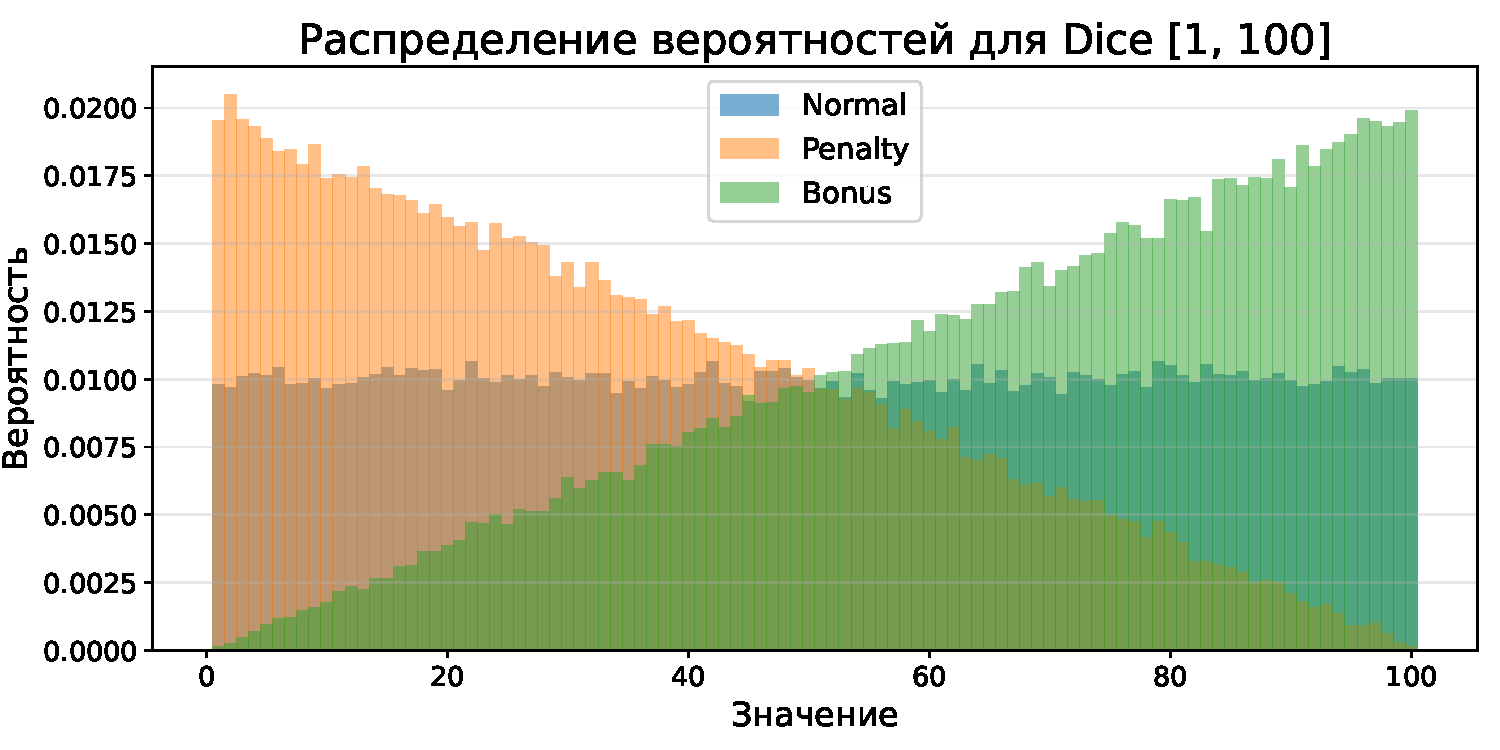
\includegraphics[width=0.9\linewidth]{dice100}
		\caption{Гистограмма вероятностей для случайной величины со значениями $[1, 100]$}

	\end{figure}
	
	\vspace{-0.5em}
	\begin{figure}[H]
		\centering
		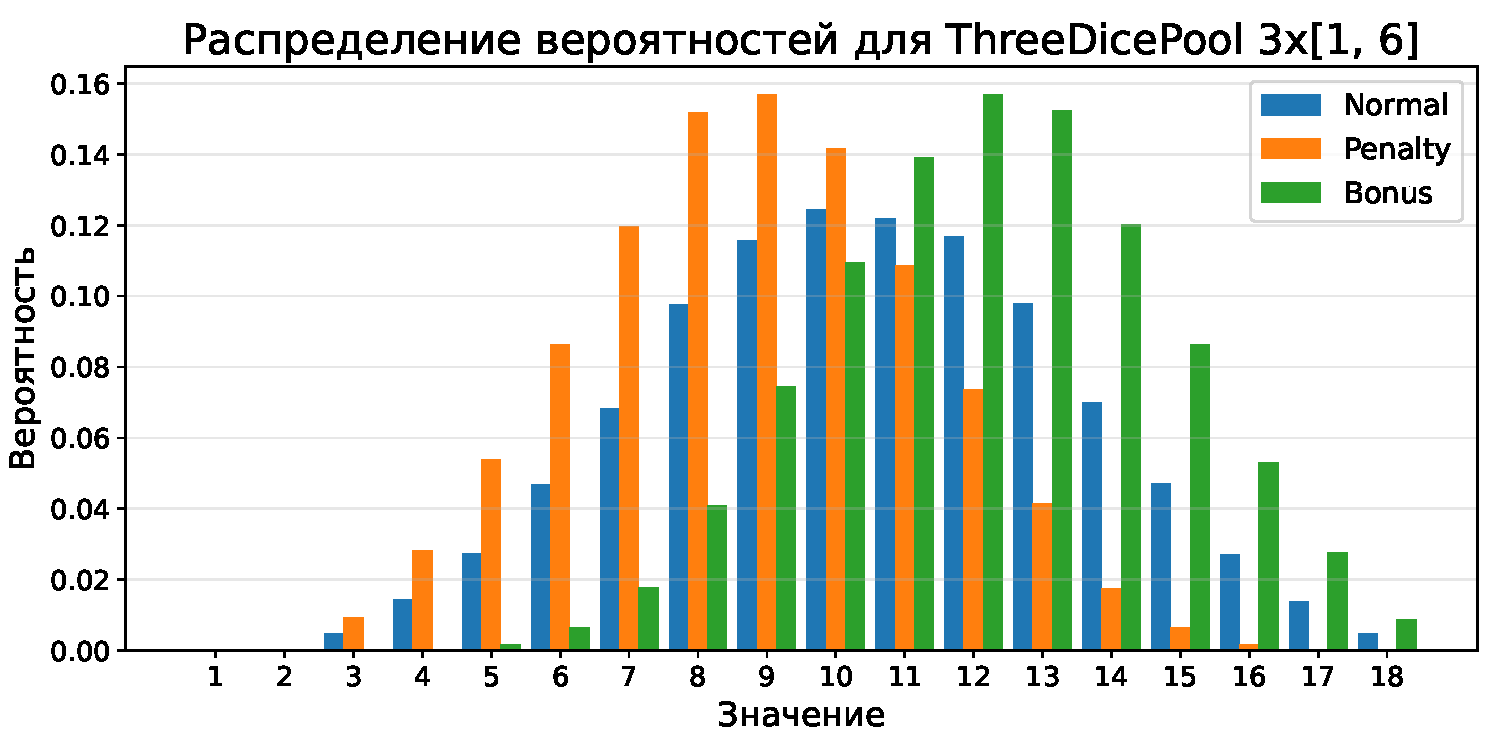
\includegraphics[width=0.9\linewidth]{pool3d6}
		\caption{Гистограмма вероятностей для \texttt{ThreeDicePool} из трёх величин со значениями $[1, 6]$}
	
	\end{figure}
	
	
	\section{Множественное наследование}
	
	Сконструирован класс \texttt{DoubleDice}, одновременно наследующий \texttt{PenaltyDice} и \texttt{BonusDice} от одной и той же случайной величины. Поскольку оба родительских класса наследуются от базового класса \texttt{Dice}, возникает ромбовидное наследование. Для устранения неоднозначности при приведении \texttt{DoubleDice} к базовому типу \texttt{Dice\&} в классах \texttt{PenaltyDice} и \texttt{BonusDice} использовано виртуальное наследование (\texttt{virtual public Dice}). Метод \texttt{roll()} в \texttt{DoubleDice} возвращает сумму \texttt{PenaltyDice::roll() + BonusDice::roll()}.
	
	Также предложена реализация \texttt{DoubleDiceComp} без множественного наследования на основе композиции: класс наследуется напрямую от \texttt{Dice} и хранит экземпляры \texttt{PenaltyDice} и \texttt{BonusDice} как приватные поля, что избавляет от ромбовидной схемы наследования.
	
	Измерения математического ожидания при $N = 100\,000$ бросков для величины со значениями $[1, 100]$ дают $\langle X \rangle \approx 101.0$ для обеих реализаций, что совпадает с теоретическим значением:
	\[
		E[\text{DoubleDice}] = E[\min(X_1, X_2)] + E[\max(X_3, X_4)] = 2 E[X] = 2 \times 50.5 = 101.
	\]
	Распределение вероятностей суммы сосредоточено на отрезке $[2, 200]$ и образует симметричный купол с максимумом в точке $101$.
	
	\vspace{-0.5em}
	\begin{figure}[H]
		\centering
		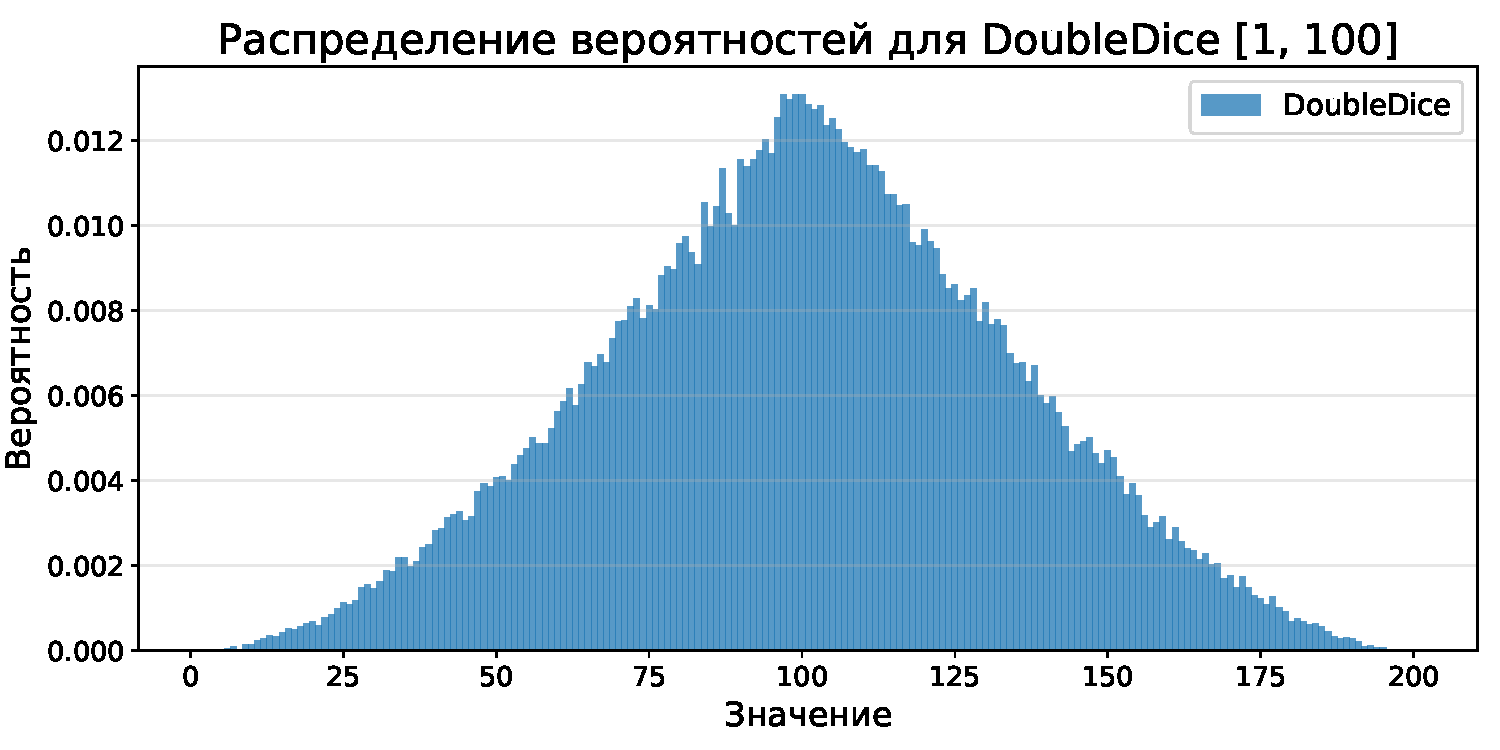
\includegraphics[width=0.9\linewidth]{double_dice}
		\caption{Гистограмма вероятностей значений для \texttt{DoubleDice} от величины со значениями $[1, 100]$}
	\end{figure}

\end{document}